\documentclass{article}
\usepackage[utf8]{inputenc}
\usepackage[a4paper, total={7in, 9in}]{geometry}
\usepackage{minted}
\usepackage{graphicx}
\usepackage{hyperref}
\usemintedstyle{manni}

\title{HPC Final}
\author{Vu Dinh Anh - m21.ict.001 }
\date{January 2023}

\begin{document}

\maketitle

\autoref{fig:original} and \autoref{fig:kuwahara} show the differences between before and after applying filter with window size of 8 (7 + 1 including the target pixel).

\begin{figure}[htbp]
    \centering
    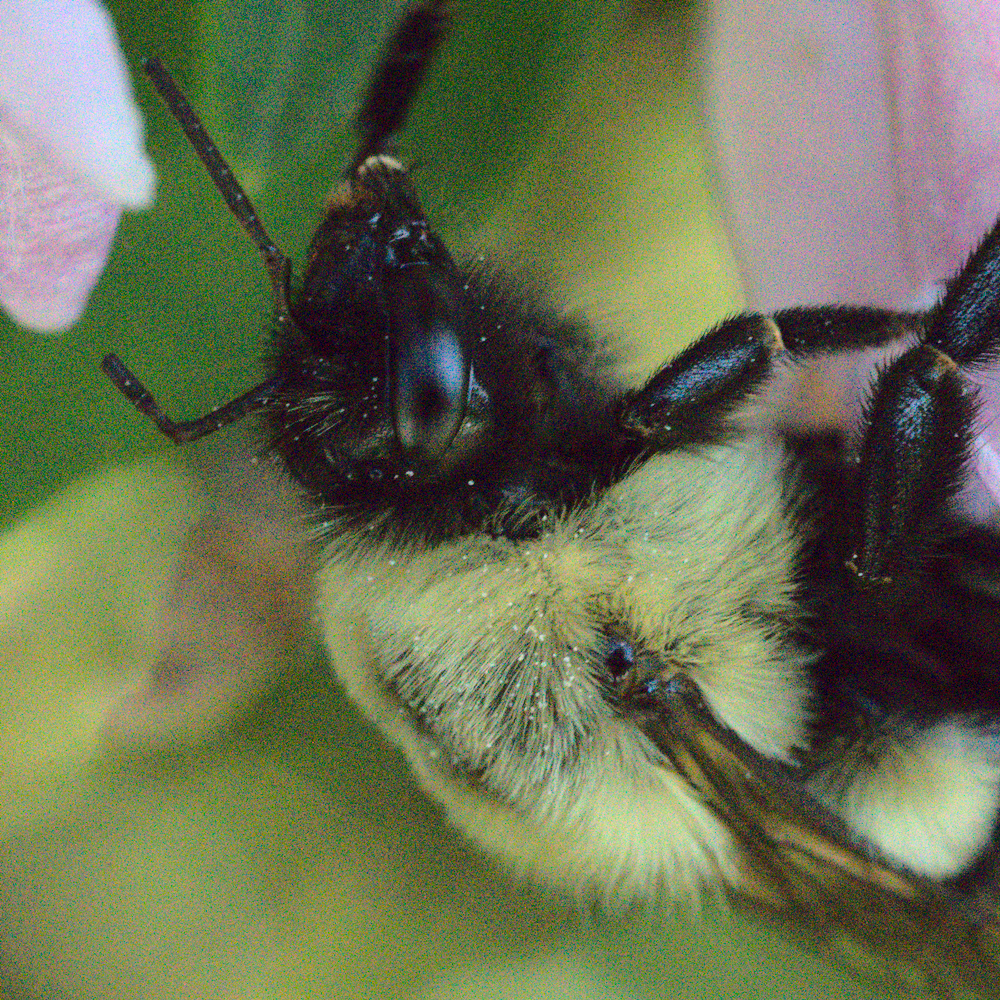
\includegraphics[scale=0.2]{in.png}
    \caption{Original image}
    \label{fig:original}
\end{figure}

\begin{figure}[htbp]
    \centering
    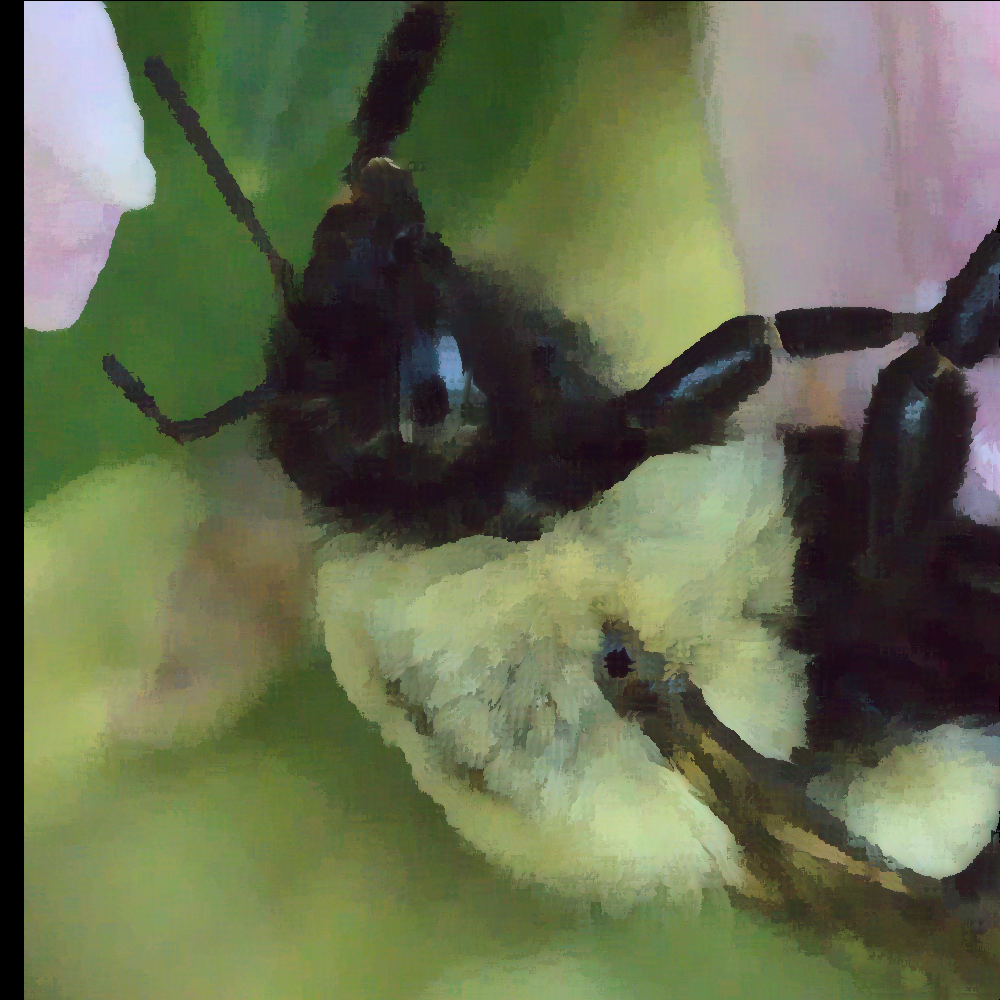
\includegraphics[scale=0.2]{out.png}
    \caption{Kuwahara filtered}
    \label{fig:kuwahara}
\end{figure}

This code was copied from previous labwork probably 8.
\begin{minted}{python}
@cuda.jit
def rgb_to_hsv(src, dst):
    i = cuda.threadIdx.x + cuda.blockIdx.x * cuda.blockDim.x
    j = cuda.threadIdx.y + cuda.blockIdx.y * cuda.blockDim.y
    r, g, b = src[i, j, 0], src[i, j, 1], src[i, j, 2]
    max_c = max(r, g, b)
    min_c = min(r, g, b)
    d = max_c - min_c
    
    # h
    if d == np.float64(0):
        dst[i, j, 0] = np.float64(0)
    if max_c == r:
        dst[i, j, 0] = 60 * ((g - b)/d % 6)
    if max_c == g:
        dst[i, j, 0] = 60 * ((b - r)/d + 2)
    if max_c == b:
        dst[i, j, 0] = 60 * ((r - g)/d + 4)
    
    # s
    if max_c == np.float64(0):
        dst[i, j, 1] = np.float64(0)
    if max_c != np.float64(0):
        dst[i, j, 1] = d/max_c
        
    # v
    dst[i, j, 2] = max_c
\end{minted}

An end-to-end function is used to package and show the step. It's not much but honest work.

\begin{minted}{python}
def e2e_rgb_to_hsv(img_in):
    img_in = np.array(img_in, copy=True)
    img_in = np.float64(img_in)
    img_in /= 255
    img_in = np.ascontiguousarray(img_in)
    h, w, c = img_in.shape
    hsv = np.array(img_in, copy=True)

    # Configure CUDA blocks
    block_size = (32, 32)
    grid_size = dual_tuple_division(block_size, (h, w))
    
    cuda_img_in = cuda.to_device(img_in)
    cuda_hsv = cuda.to_device(hsv)
    
    rgb_to_hsv[grid_size, block_size](cuda_img_in, cuda_hsv)
    hsv = cuda_hsv.copy_to_host()
    return hsv
\end{minted}

I implemented Kuwahara filter poorly. Each window's standard deviation is implemented manually. Then I find minimum standard deiviation. Laslty I check min std manually. It's not a good solution.
\begin{minted}{python}
@cuda.jit
def kuwahara_filter(rgb_src, rgb_dst, v_arr, window_size):
    i = cuda.threadIdx.x + cuda.blockIdx.x * cuda.blockDim.x
    j = cuda.threadIdx.y + cuda.blockIdx.y * cuda.blockDim.y
    height, width = v_arr.shape
    
    # window 0
    sum_ = np.float64(0)
    sum_power_2 = np.float64(0)
    for wi in range(i - window_size, i):
        for wj in range(j - window_size, j):
            if wi >= 0 and wi < height and wj >= 0 and wj < width:
                sum_ += v_arr[wi, wj]
                sum_power_2 += v_arr[wi, wj] * v_arr[wi, wj]
            
    mean_ = sum_ / (window_size * window_size)
    std_window_0 = math.sqrt(sum_power_2 / (window_size * window_size) - mean_ * mean_)
    
    # window 1
    sum_ = np.float64(0)
    sum_power_2 = np.float64(0)
    for wi in range(i, i + window_size):
        for wj in range(j - window_size, j):
            if wi >= 0 and wi < height and wj >= 0 and wj < width:
                sum_ += v_arr[wi, wj]
                sum_power_2 += v_arr[wi, wj] * v_arr[wi, wj]
            
    mean_ = sum_ / (window_size * window_size)
    std_window_1 = math.sqrt(sum_power_2 / (window_size * window_size) - mean_ * mean_)
    
    # window 2
    sum_ = np.float64(0)
    sum_power_2 = np.float64(0)
    for wi in range(i - window_size, i):
        for wj in range(j, j + window_size):
            if wi >= 0 and wi < height and wj >= 0 and wj < width:
                sum_ += v_arr[wi, wj]
                sum_power_2 += v_arr[wi, wj] * v_arr[wi, wj]
            
    mean_ = sum_ / (window_size * window_size)
    std_window_2 = math.sqrt(sum_power_2 / (window_size * window_size) - mean_ * mean_)
    
    # window 3
    sum_ = np.float64(0)
    sum_power_2 = np.float64(0)
    for wi in range(i, i + window_size):
        for wj in range(j, j + window_size):
            if wi >= 0 and wi < height and wj >= 0 and wj < width:
                sum_ += v_arr[wi, wj]
                sum_power_2 += v_arr[wi, wj] * v_arr[wi, wj]
            
    mean_ = sum_ / (window_size * window_size)
    std_window_3 = math.sqrt(sum_power_2 / (window_size * window_size) - mean_ * mean_)
    
    # find min std
    min_std = min(std_window_0, std_window_1, std_window_2, std_window_3)
    
    # assign avg rgb of window to the target pixel
    avg_r = np.float64(0.0)
    avg_g = np.float64(0.0)
    avg_b = np.float64(0.0)
    if min_std == std_window_0:
        # window 0
        for wi in range(i- window_size, i):
            for wj in range(j - window_size, j):
                if wi >= 0 and wi < height and wj >= 0 and wj < width:
                    avg_r += rgb_src[wi, wj, 0]
                    avg_g += rgb_src[wi, wj, 1]
                    avg_b += rgb_src[wi, wj, 2]
                
    elif min_std == std_window_1:
        # window 1
        for wi in range(i, i + window_size):
            for wj in range(j - window_size, j):
                if wi >= 0 and wi < height and wj >= 0 and wj < width:
                    avg_r += rgb_src[wi, wj, 0]
                    avg_g += rgb_src[wi, wj, 1]
                    avg_b += rgb_src[wi, wj, 2]
    elif min_std == std_window_2:
        # window 2
        for wi in range(i - window_size, i):
            for wj in range(j, j + window_size):
                if wi >= 0 and wi < height and wj >= 0 and wj < width:
                    avg_r += rgb_src[wi, wj, 0]
                    avg_g += rgb_src[wi, wj, 1]
                    avg_b += rgb_src[wi, wj, 2]
    else:
        # window 3
        for wi in range(i, i + window_size):
            for wj in range(j, j + window_size):
                if wi >= 0 and wi < height and wj >= 0 and wj < width:
                    avg_r += rgb_src[wi, wj, 0]
                    avg_g += rgb_src[wi, wj, 1]
                    avg_b += rgb_src[wi, wj, 2]
    
    avg_r = np.uint8(avg_r / (window_size * window_size))
    avg_g = np.uint8(avg_g / (window_size * window_size))
    avg_b = np.uint8(avg_b / (window_size * window_size))
    
    rgb_dst[i, j, 0] = avg_r
    rgb_dst[i, j, 1] = avg_g
    rgb_dst[i, j, 2] = avg_b

\end{minted}

\subsection{Without shared memory}
\begin{minted}{text}
runtime @ block size
0.00025529870006266717 @ (2, 2)
0.00025514400001611646 @ (4, 4)
0.00026532719998613176 @ (8, 8)
0.00026966600003106576 @ (16, 16)
0.00024621869999919 @ (32, 32)
\end{minted}
\subsection{With shared memory}
I'm too tired and exhausted. Therefore, I haven't got time to implement this. Some ways are:
\begin{itemize}
    \item load rgb source image, or rgb destination image or the v channel of rgb-2-hsv converted image
    \item the value of the v channel after raised power to 2
\end{itemize}

\end{document}
